\documentclass[]{article}
\usepackage{lmodern}
\usepackage{amssymb,amsmath}
\usepackage{ifxetex,ifluatex}
\usepackage{fixltx2e} % provides \textsubscript
\ifnum 0\ifxetex 1\fi\ifluatex 1\fi=0 % if pdftex
  \usepackage[T1]{fontenc}
  \usepackage[utf8]{inputenc}
\else % if luatex or xelatex
  \ifxetex
    \usepackage{mathspec}
  \else
    \usepackage{fontspec}
  \fi
  \defaultfontfeatures{Ligatures=TeX,Scale=MatchLowercase}
\fi
% use upquote if available, for straight quotes in verbatim environments
\IfFileExists{upquote.sty}{\usepackage{upquote}}{}
% use microtype if available
\IfFileExists{microtype.sty}{%
\usepackage{microtype}
\UseMicrotypeSet[protrusion]{basicmath} % disable protrusion for tt fonts
}{}
\usepackage[margin=1in]{geometry}
\usepackage{hyperref}
\hypersetup{unicode=true,
            pdftitle={ps1\_q3},
            pdfauthor={Sijun Zhang},
            pdfborder={0 0 0},
            breaklinks=true}
\urlstyle{same}  % don't use monospace font for urls
\usepackage{color}
\usepackage{fancyvrb}
\newcommand{\VerbBar}{|}
\newcommand{\VERB}{\Verb[commandchars=\\\{\}]}
\DefineVerbatimEnvironment{Highlighting}{Verbatim}{commandchars=\\\{\}}
% Add ',fontsize=\small' for more characters per line
\usepackage{framed}
\definecolor{shadecolor}{RGB}{248,248,248}
\newenvironment{Shaded}{\begin{snugshade}}{\end{snugshade}}
\newcommand{\AlertTok}[1]{\textcolor[rgb]{0.94,0.16,0.16}{#1}}
\newcommand{\AnnotationTok}[1]{\textcolor[rgb]{0.56,0.35,0.01}{\textbf{\textit{#1}}}}
\newcommand{\AttributeTok}[1]{\textcolor[rgb]{0.77,0.63,0.00}{#1}}
\newcommand{\BaseNTok}[1]{\textcolor[rgb]{0.00,0.00,0.81}{#1}}
\newcommand{\BuiltInTok}[1]{#1}
\newcommand{\CharTok}[1]{\textcolor[rgb]{0.31,0.60,0.02}{#1}}
\newcommand{\CommentTok}[1]{\textcolor[rgb]{0.56,0.35,0.01}{\textit{#1}}}
\newcommand{\CommentVarTok}[1]{\textcolor[rgb]{0.56,0.35,0.01}{\textbf{\textit{#1}}}}
\newcommand{\ConstantTok}[1]{\textcolor[rgb]{0.00,0.00,0.00}{#1}}
\newcommand{\ControlFlowTok}[1]{\textcolor[rgb]{0.13,0.29,0.53}{\textbf{#1}}}
\newcommand{\DataTypeTok}[1]{\textcolor[rgb]{0.13,0.29,0.53}{#1}}
\newcommand{\DecValTok}[1]{\textcolor[rgb]{0.00,0.00,0.81}{#1}}
\newcommand{\DocumentationTok}[1]{\textcolor[rgb]{0.56,0.35,0.01}{\textbf{\textit{#1}}}}
\newcommand{\ErrorTok}[1]{\textcolor[rgb]{0.64,0.00,0.00}{\textbf{#1}}}
\newcommand{\ExtensionTok}[1]{#1}
\newcommand{\FloatTok}[1]{\textcolor[rgb]{0.00,0.00,0.81}{#1}}
\newcommand{\FunctionTok}[1]{\textcolor[rgb]{0.00,0.00,0.00}{#1}}
\newcommand{\ImportTok}[1]{#1}
\newcommand{\InformationTok}[1]{\textcolor[rgb]{0.56,0.35,0.01}{\textbf{\textit{#1}}}}
\newcommand{\KeywordTok}[1]{\textcolor[rgb]{0.13,0.29,0.53}{\textbf{#1}}}
\newcommand{\NormalTok}[1]{#1}
\newcommand{\OperatorTok}[1]{\textcolor[rgb]{0.81,0.36,0.00}{\textbf{#1}}}
\newcommand{\OtherTok}[1]{\textcolor[rgb]{0.56,0.35,0.01}{#1}}
\newcommand{\PreprocessorTok}[1]{\textcolor[rgb]{0.56,0.35,0.01}{\textit{#1}}}
\newcommand{\RegionMarkerTok}[1]{#1}
\newcommand{\SpecialCharTok}[1]{\textcolor[rgb]{0.00,0.00,0.00}{#1}}
\newcommand{\SpecialStringTok}[1]{\textcolor[rgb]{0.31,0.60,0.02}{#1}}
\newcommand{\StringTok}[1]{\textcolor[rgb]{0.31,0.60,0.02}{#1}}
\newcommand{\VariableTok}[1]{\textcolor[rgb]{0.00,0.00,0.00}{#1}}
\newcommand{\VerbatimStringTok}[1]{\textcolor[rgb]{0.31,0.60,0.02}{#1}}
\newcommand{\WarningTok}[1]{\textcolor[rgb]{0.56,0.35,0.01}{\textbf{\textit{#1}}}}
\usepackage{graphicx,grffile}
\makeatletter
\def\maxwidth{\ifdim\Gin@nat@width>\linewidth\linewidth\else\Gin@nat@width\fi}
\def\maxheight{\ifdim\Gin@nat@height>\textheight\textheight\else\Gin@nat@height\fi}
\makeatother
% Scale images if necessary, so that they will not overflow the page
% margins by default, and it is still possible to overwrite the defaults
% using explicit options in \includegraphics[width, height, ...]{}
\setkeys{Gin}{width=\maxwidth,height=\maxheight,keepaspectratio}
\IfFileExists{parskip.sty}{%
\usepackage{parskip}
}{% else
\setlength{\parindent}{0pt}
\setlength{\parskip}{6pt plus 2pt minus 1pt}
}
\setlength{\emergencystretch}{3em}  % prevent overfull lines
\providecommand{\tightlist}{%
  \setlength{\itemsep}{0pt}\setlength{\parskip}{0pt}}
\setcounter{secnumdepth}{0}
% Redefines (sub)paragraphs to behave more like sections
\ifx\paragraph\undefined\else
\let\oldparagraph\paragraph
\renewcommand{\paragraph}[1]{\oldparagraph{#1}\mbox{}}
\fi
\ifx\subparagraph\undefined\else
\let\oldsubparagraph\subparagraph
\renewcommand{\subparagraph}[1]{\oldsubparagraph{#1}\mbox{}}
\fi

%%% Use protect on footnotes to avoid problems with footnotes in titles
\let\rmarkdownfootnote\footnote%
\def\footnote{\protect\rmarkdownfootnote}

%%% Change title format to be more compact
\usepackage{titling}

% Create subtitle command for use in maketitle
\providecommand{\subtitle}[1]{
  \posttitle{
    \begin{center}\large#1\end{center}
    }
}

\setlength{\droptitle}{-2em}

  \title{ps1\_q3}
    \pretitle{\vspace{\droptitle}\centering\huge}
  \posttitle{\par}
    \author{Sijun Zhang}
    \preauthor{\centering\large\emph}
  \postauthor{\par}
      \predate{\centering\large\emph}
  \postdate{\par}
    \date{2019/9/23}


\begin{document}
\maketitle

\hypertarget{problem-3}{%
\section{Problem 3}\label{problem-3}}

\hypertarget{import-data}{%
\subsection{Import Data}\label{import-data}}

\begin{Shaded}
\begin{Highlighting}[]
\NormalTok{traj <-}\StringTok{ }\KeywordTok{read.table}\NormalTok{(}\StringTok{'train_trajectories.csv'}\NormalTok{, }\DataTypeTok{sep =} \StringTok{','}\NormalTok{, }\DataTypeTok{stringsAsFactors =} \OtherTok{FALSE}\NormalTok{, }\DataTypeTok{header =} \OtherTok{TRUE}\NormalTok{)}
\NormalTok{traj_}\DecValTok{01}\NormalTok{_}\DecValTok{04}\NormalTok{ <-}\StringTok{ }\NormalTok{traj[(traj}\OperatorTok{$}\NormalTok{subject_nr }\OperatorTok{==}\StringTok{ }\DecValTok{1}\NormalTok{) }\OperatorTok{&}\StringTok{ }\NormalTok{(traj}\OperatorTok{$}\NormalTok{count_trial }\OperatorTok{==}\StringTok{ }\DecValTok{4}\NormalTok{), }\DecValTok{3}\OperatorTok{:}\DecValTok{5}\NormalTok{]}
\NormalTok{traj_m <-}\StringTok{ }\KeywordTok{as.matrix}\NormalTok{(traj_}\DecValTok{01}\NormalTok{_}\DecValTok{04}\NormalTok{)}
\KeywordTok{plot}\NormalTok{(traj_m[, }\DecValTok{1}\NormalTok{], traj_m[, }\DecValTok{2}\NormalTok{])}
\end{Highlighting}
\end{Shaded}

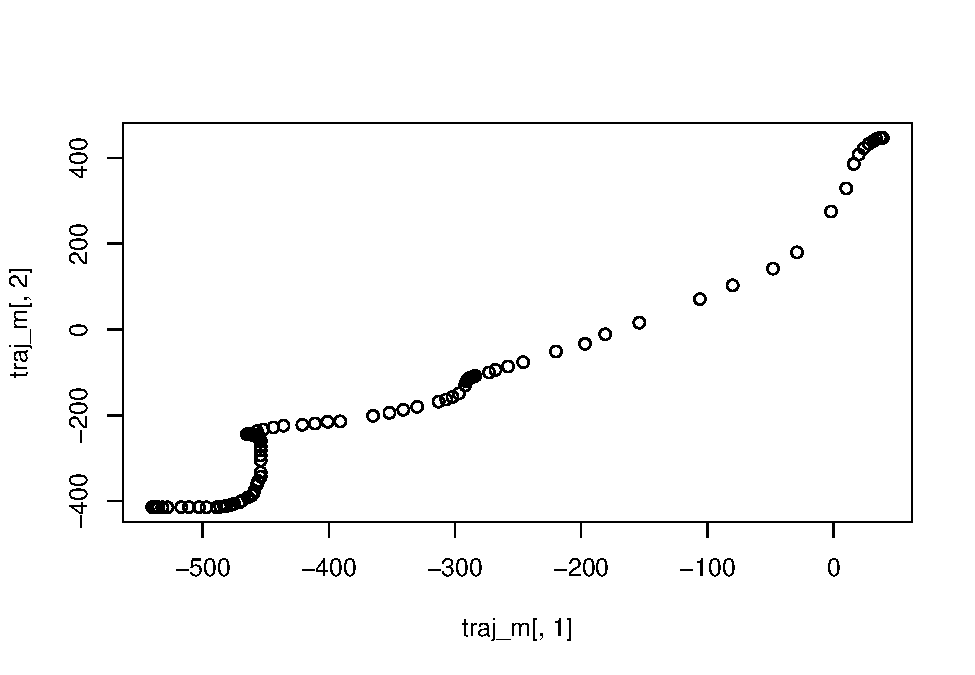
\includegraphics{ps1_q3_files/figure-latex/unnamed-chunk-1-1.pdf}

\hypertarget{set-origin-zero}{%
\subsection{Set Origin Zero}\label{set-origin-zero}}

{[}5pts{]} Write a function that accepts a n n×3 matrix representing the
trajectory (x, y, t) and translates it to begin with time zero at the
origin.

\begin{Shaded}
\begin{Highlighting}[]
\CommentTok{# INPUT: n×3 matrix representing the trajectory (x, y, t)}
\CommentTok{# OUTPUT: nx3 matrix begining with time zero at the origin}
\NormalTok{set_origin_zero =}\StringTok{ }\ControlFlowTok{function}\NormalTok{(x) \{}
\NormalTok{  n <-}\StringTok{ }\KeywordTok{dim}\NormalTok{(x)[}\DecValTok{1}\NormalTok{]}
\NormalTok{  origin <-}\StringTok{ }\NormalTok{x[}\DecValTok{1}\NormalTok{,]}
\NormalTok{  y <-}\StringTok{ }\NormalTok{x}
  \ControlFlowTok{for}\NormalTok{ (i }\ControlFlowTok{in} \DecValTok{1}\OperatorTok{:}\NormalTok{n) \{}
\NormalTok{    y[i,] <-}\StringTok{ }\NormalTok{y[i,] }\OperatorTok{-}\StringTok{ }\NormalTok{origin}
\NormalTok{  \}}
  \KeywordTok{return}\NormalTok{(y)}
\NormalTok{\}}
\NormalTok{traj_m <-}\StringTok{ }\KeywordTok{set_origin_zero}\NormalTok{(traj_m)}
\KeywordTok{plot}\NormalTok{(traj_m[, }\DecValTok{1}\NormalTok{], traj_m[, }\DecValTok{2}\NormalTok{])}
\end{Highlighting}
\end{Shaded}

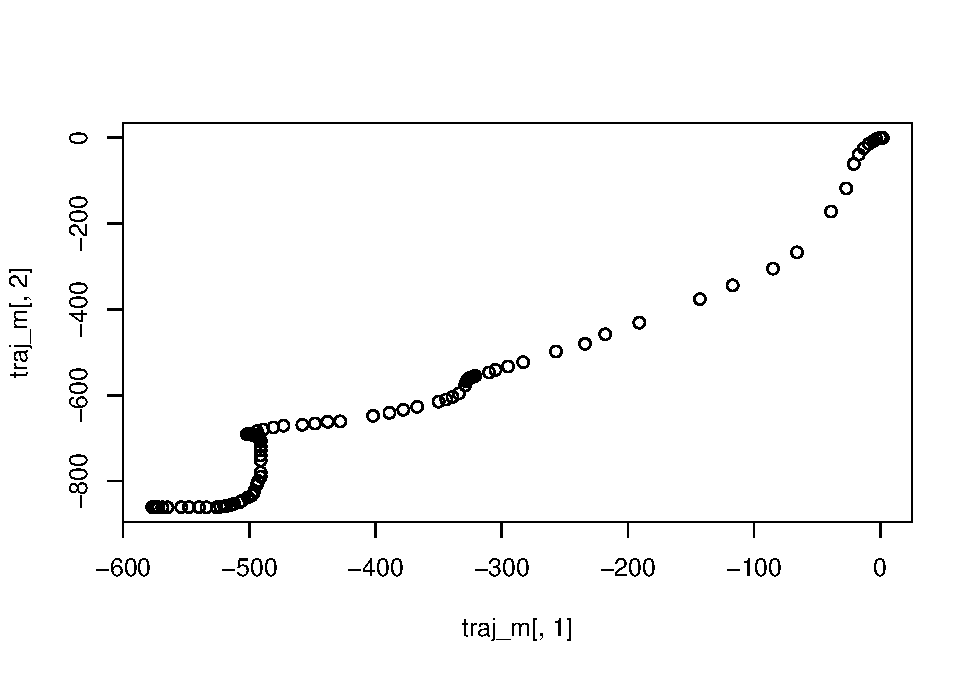
\includegraphics{ps1_q3_files/figure-latex/unnamed-chunk-2-1.pdf}

In this part, I sequentially minused each point with the origin
coordination, so that the curve was translated to the one beginning at
origin and time zero.

\hypertarget{compute-angle}{%
\subsection{Compute Angle}\label{compute-angle}}

{[}5pts{]} Write a function that computes the angle θ formed by the
secant line connecting the origin and the final position in the
trajectory. Your answer should be an angle between {[}−π,π{]}. Be sure
your your solution works for a trajectory ending in any of the four
quadrants.

\begin{Shaded}
\begin{Highlighting}[]
\CommentTok{# INPUT: xops and yops value of a point}
\CommentTok{# OUTPUT: the angle θ formed by the line connecting the origin and the point}
\NormalTok{compute_angle =}\StringTok{ }\ControlFlowTok{function}\NormalTok{(x, y) \{}
  \ControlFlowTok{if}\NormalTok{ (x }\OperatorTok{==}\StringTok{ }\DecValTok{0}\NormalTok{) \{}
    \ControlFlowTok{if}\NormalTok{ (y }\OperatorTok{==}\StringTok{ }\DecValTok{0}\NormalTok{) \{theta <-}\StringTok{ }\DecValTok{0}\NormalTok{\}}
    \ControlFlowTok{else}\NormalTok{ \{}
\NormalTok{      theta <-}\StringTok{ }\KeywordTok{sign}\NormalTok{(y) }\OperatorTok{*}\StringTok{ }\NormalTok{(}\DecValTok{1} \OperatorTok{/}\StringTok{ }\DecValTok{2}\NormalTok{) }\OperatorTok{*}\StringTok{ }\NormalTok{pi}
\NormalTok{    \}}
\NormalTok{  \}}
  \ControlFlowTok{else} \ControlFlowTok{if}\NormalTok{ (x }\OperatorTok{>}\StringTok{ }\DecValTok{0}\NormalTok{) \{ }
\NormalTok{    theta <-}\StringTok{ }\KeywordTok{atan}\NormalTok{(y }\OperatorTok{/}\StringTok{ }\NormalTok{x)}
\NormalTok{  \}}
  \ControlFlowTok{else}\NormalTok{ \{}
\NormalTok{    tmp <-}\StringTok{ }\KeywordTok{atan}\NormalTok{(y }\OperatorTok{/}\StringTok{ }\NormalTok{x)}
\NormalTok{    theta <-}\StringTok{ }\NormalTok{tmp }\OperatorTok{-}\StringTok{ }\KeywordTok{sign}\NormalTok{(tmp) }\OperatorTok{*}\StringTok{ }\NormalTok{pi}
    \ControlFlowTok{if}\NormalTok{ (y }\OperatorTok{==}\StringTok{ }\DecValTok{0}\NormalTok{) \{}
\NormalTok{      theta <-}\StringTok{ }\OperatorTok{-}\NormalTok{pi}
\NormalTok{    \}}
\NormalTok{  \}}
  \KeywordTok{names}\NormalTok{(theta) <-}\StringTok{ }\OtherTok{NULL}
  \KeywordTok{return}\NormalTok{(theta)}
\NormalTok{\}}

\CommentTok{# INPUT: n×3 matrix representing the trajectory (x, y, t) beginning at zero}
\CommentTok{# OUTPUT: the angle θ formed by the secant line connecting the origin and the final position in the trajectory}
\NormalTok{compute_secant_angle =}\StringTok{ }\ControlFlowTok{function}\NormalTok{(x) \{}
\NormalTok{  n <-}\StringTok{ }\KeywordTok{dim}\NormalTok{(x)[}\DecValTok{1}\NormalTok{]}
\NormalTok{  final <-}\StringTok{ }\NormalTok{x[n,]}
\NormalTok{  final_x <-}\StringTok{ }\NormalTok{final[}\DecValTok{1}\NormalTok{]}
\NormalTok{  final_y <-}\StringTok{ }\NormalTok{final[}\DecValTok{2}\NormalTok{]}
\NormalTok{  theta <-}\StringTok{ }\KeywordTok{compute_angle}\NormalTok{(final_x, final_y)}
  \KeywordTok{return}\NormalTok{(theta)}
\NormalTok{\}}
\KeywordTok{compute_secant_angle}\NormalTok{(traj_m)}
\end{Highlighting}
\end{Shaded}

\begin{verbatim}
## [1] -2.161207
\end{verbatim}

In this part, I wrote a universal function to compute the angle between
the origin and the selected pint. I found that the period of tan
function is only π, there were two special cases need to aware, one is
the points at 3rd and 2nd quadrants and the other one is the points
lying on the negative axis. I set the the points lying on the negative
axis have -π angle to avoid runtime error.

\hypertarget{rotate-end-to-x-axis}{%
\subsection{Rotate End to X-axis}\label{rotate-end-to-x-axis}}

{[}5pts{]} Write a function to rotate the (x, y) coordinates of a
trajectory so that the final point lies along the positive x-axis.

\begin{Shaded}
\begin{Highlighting}[]
\CommentTok{# INPUT: n×3 matrix representing the trajectory (x, y, t) beginning at zero}
\CommentTok{# OUTPUT: rotate the (x, y) coordinates of a trajectory so that the final point lies along the positive x-axis.}
\NormalTok{rotate_end_to_xaxis =}\StringTok{ }\ControlFlowTok{function}\NormalTok{(x) \{}
\NormalTok{  n <-}\StringTok{ }\KeywordTok{dim}\NormalTok{(x)[}\DecValTok{1}\NormalTok{]}
\NormalTok{  y <-}\StringTok{ }\NormalTok{x}
\NormalTok{  theta <-}\StringTok{ }\KeywordTok{compute_secant_angle}\NormalTok{(x)}
  \ControlFlowTok{for}\NormalTok{ (i }\ControlFlowTok{in} \DecValTok{1}\OperatorTok{:}\NormalTok{n) \{}
\NormalTok{    theta_i <-}\StringTok{ }\KeywordTok{compute_angle}\NormalTok{(x[i, }\DecValTok{1}\NormalTok{], x[i, }\DecValTok{2}\NormalTok{])}
\NormalTok{    theta_i <-}\StringTok{ }\NormalTok{theta_i }\OperatorTok{-}\StringTok{ }\NormalTok{theta}
\NormalTok{    secant_distance <-}\StringTok{ }\KeywordTok{sqrt}\NormalTok{(x[i, }\DecValTok{1}\NormalTok{]}\OperatorTok{^}\DecValTok{2} \OperatorTok{+}\StringTok{ }\NormalTok{x[i, }\DecValTok{2}\NormalTok{]}\OperatorTok{^}\DecValTok{2}\NormalTok{)}
\NormalTok{    y[i,}\DecValTok{1}\NormalTok{] <-}\StringTok{ }\NormalTok{secant_distance }\OperatorTok{*}\StringTok{ }\KeywordTok{cos}\NormalTok{(theta_i)}
\NormalTok{    y[i,}\DecValTok{2}\NormalTok{] <-}\StringTok{ }\NormalTok{secant_distance }\OperatorTok{*}\StringTok{ }\KeywordTok{sin}\NormalTok{(theta_i)}
\NormalTok{  \}}
  \KeywordTok{return}\NormalTok{(y)}
\NormalTok{\}}
\NormalTok{traj_m <-}\StringTok{ }\KeywordTok{set_origin_zero}\NormalTok{(traj_m)}
\NormalTok{traj_m <-}\StringTok{ }\KeywordTok{rotate_end_to_xaxis}\NormalTok{(traj_m)}
\KeywordTok{plot}\NormalTok{(traj_m[, }\DecValTok{1}\NormalTok{], traj_m[, }\DecValTok{2}\NormalTok{])}
\end{Highlighting}
\end{Shaded}

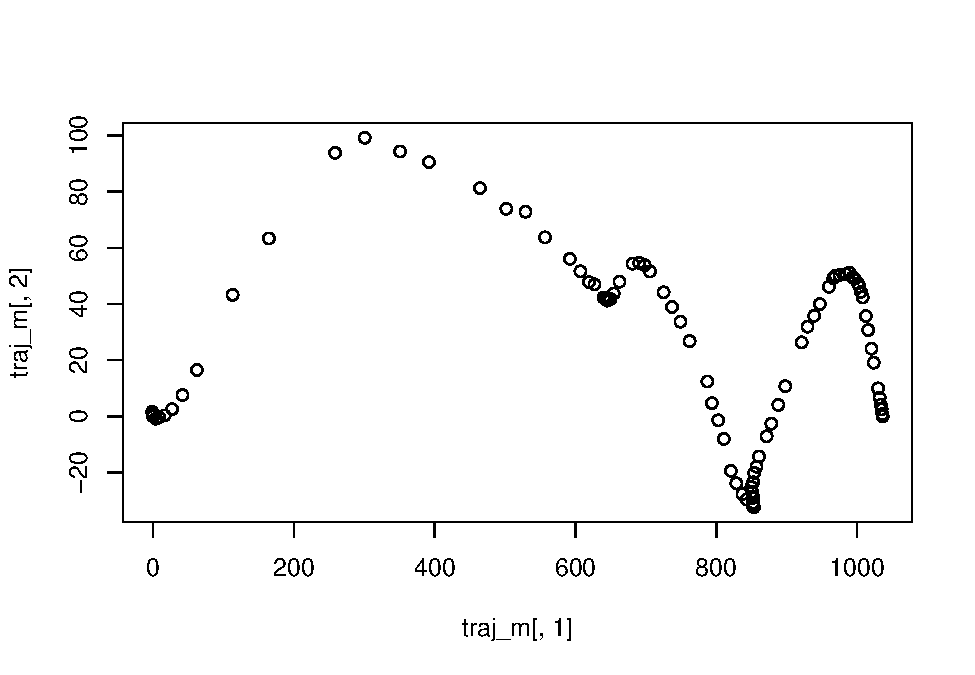
\includegraphics{ps1_q3_files/figure-latex/unnamed-chunk-4-1.pdf}

In this part, I computed each point's angle to the origin and minus the
angle of the last points, then maintain the secant distance unchanged to
rotate each point to the new angle, so that the curve was rotated to
have the ends on x-axis.

\hypertarget{normalize}{%
\subsection{Normalize}\label{normalize}}

{[}2pts{]} Combine the three parts above into a single function that
normalizes an n×3 trajectory matrix to begin at the origin and end on
the positive x-axis.

\begin{Shaded}
\begin{Highlighting}[]
\CommentTok{# INPUT: n×3 matrix representing the trajectory (x, y, t)}
\CommentTok{# OUTPUT: rotate the (x, y) coordinates of a trajectory so that the final point lies along the positive x-axis.}
\NormalTok{normalize =}\StringTok{ }\ControlFlowTok{function}\NormalTok{(x) \{}
\NormalTok{  y <-}\StringTok{ }\KeywordTok{set_origin_zero}\NormalTok{(x)}
\NormalTok{  y <-}\StringTok{ }\KeywordTok{rotate_end_to_xaxis}\NormalTok{(y)}
  \KeywordTok{return}\NormalTok{(y)}
\NormalTok{\}}
\NormalTok{traj_m <-}\StringTok{ }\KeywordTok{normalize}\NormalTok{(traj_m)}
\KeywordTok{plot}\NormalTok{(traj_m[, }\DecValTok{1}\NormalTok{], traj_m[, }\DecValTok{2}\NormalTok{])}
\end{Highlighting}
\end{Shaded}

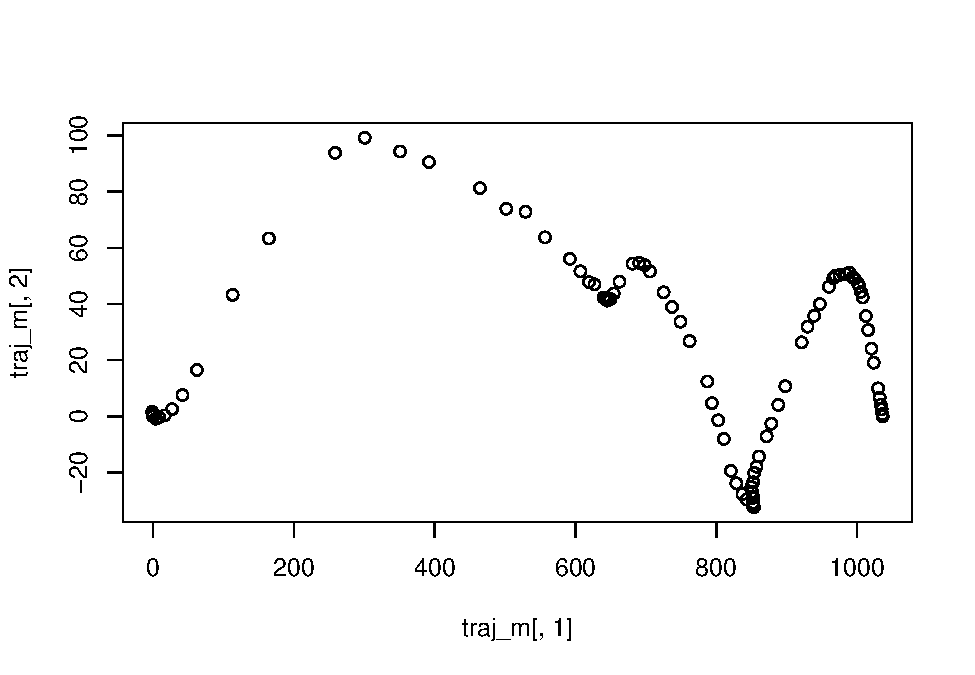
\includegraphics{ps1_q3_files/figure-latex/unnamed-chunk-5-1.pdf}

This part combine the previous functions into a pipeline.

\hypertarget{measure-the-curvature}{%
\subsection{Measure the Curvature}\label{measure-the-curvature}}

{[}8pts{]} Write a function that accepts a normalized trajectory and
computes the following metrics describing its curvature:

\begin{Shaded}
\begin{Highlighting}[]
\CommentTok{# INPUT: a normalized trajectory}
\CommentTok{# OUTPUT:  the metrics describing its curvature }
\NormalTok{measure_curvature =}\StringTok{ }\ControlFlowTok{function}\NormalTok{(x) \{}
  \CommentTok{# Calc the total (Euclidean) distance traveled}
\NormalTok{  n <-}\StringTok{ }\KeywordTok{dim}\NormalTok{(x)[}\DecValTok{1}\NormalTok{]}
\NormalTok{  tot_dist <-}\StringTok{ }\DecValTok{0}
  \ControlFlowTok{for}\NormalTok{ (i }\ControlFlowTok{in} \DecValTok{1}\OperatorTok{:}\NormalTok{(n }\OperatorTok{-}\StringTok{ }\DecValTok{1}\NormalTok{)) \{}
\NormalTok{    dist_i <-}\StringTok{ }\KeywordTok{sqrt}\NormalTok{((x[i, }\DecValTok{1}\NormalTok{] }\OperatorTok{-}\StringTok{ }\NormalTok{x[i }\OperatorTok{+}\StringTok{ }\DecValTok{1}\NormalTok{, }\DecValTok{1}\NormalTok{])}\OperatorTok{^}\DecValTok{2} \OperatorTok{+}\StringTok{ }\NormalTok{(x[i, }\DecValTok{2}\NormalTok{] }\OperatorTok{-}\StringTok{ }\NormalTok{x[i }\OperatorTok{+}\StringTok{ }\DecValTok{1}\NormalTok{, }\DecValTok{2}\NormalTok{])}\OperatorTok{^}\DecValTok{2}\NormalTok{)}
\NormalTok{    tot_dist <-}\StringTok{ }\NormalTok{dist_i }\OperatorTok{+}\StringTok{ }\NormalTok{tot_dist}
\NormalTok{  \}}
  
  \CommentTok{# Calc the maximum absolute deviation from the secant connecting the starting and final positions}
\NormalTok{  max_abs_dev <-}\StringTok{ }\KeywordTok{max}\NormalTok{(}\KeywordTok{abs}\NormalTok{(x[, }\DecValTok{2}\NormalTok{])) }
  
  \CommentTok{# Calc the average absolute deviation of the observed trajectory from the direct path}
\NormalTok{  avg_abs_dev <-}\StringTok{ }\KeywordTok{mean}\NormalTok{(}\KeywordTok{abs}\NormalTok{(x[, }\DecValTok{2}\NormalTok{]))}
  
  \CommentTok{# Calc the (absolute) area under the curve for the trajectory relative to the secant line using the trapezoidal rule to integrate}
\NormalTok{  AUC <-}\StringTok{ }\DecValTok{0}
  \ControlFlowTok{for}\NormalTok{ (i }\ControlFlowTok{in} \DecValTok{1}\OperatorTok{:}\NormalTok{(n }\OperatorTok{-}\StringTok{ }\DecValTok{1}\NormalTok{)) \{}
\NormalTok{    x_dist <-}\StringTok{ }\NormalTok{x[i }\OperatorTok{+}\StringTok{ }\DecValTok{1}\NormalTok{, }\DecValTok{1}\NormalTok{] }\OperatorTok{-}\StringTok{ }\NormalTok{x[i, }\DecValTok{1}\NormalTok{]}
\NormalTok{    AUC_i <-}\StringTok{ }\NormalTok{(}\DecValTok{1} \OperatorTok{/}\StringTok{ }\DecValTok{2}\NormalTok{) }\OperatorTok{*}\StringTok{ }\NormalTok{x_dist }\OperatorTok{*}\StringTok{ }\NormalTok{(}\KeywordTok{abs}\NormalTok{(x[i }\OperatorTok{+}\StringTok{ }\DecValTok{1}\NormalTok{, }\DecValTok{2}\NormalTok{]) }\OperatorTok{+}\StringTok{ }\KeywordTok{abs}\NormalTok{(x[i, }\DecValTok{2}\NormalTok{]))}
\NormalTok{    AUC <-}\StringTok{ }\NormalTok{AUC }\OperatorTok{+}\StringTok{ }\NormalTok{AUC_i}
\NormalTok{  \}}
\NormalTok{  re <-}\StringTok{ }\KeywordTok{c}\NormalTok{(tot_dist, max_abs_dev, avg_abs_dev, AUC)}
  \KeywordTok{return}\NormalTok{(re)}
\NormalTok{\}}
\NormalTok{traj_m <-}\StringTok{ }\KeywordTok{normalize}\NormalTok{(traj_m)}
\NormalTok{re <-}\StringTok{ }\KeywordTok{measure_curvature}\NormalTok{(traj_m)}
\KeywordTok{print}\NormalTok{(re)}
\end{Highlighting}
\end{Shaded}

\begin{verbatim}
## [1]  1153.46372    99.18373    18.17234 54516.01033
\end{verbatim}

In this part, the total (Euclidean) distance traveled, and AUC need to
traverse the curve and as the curve has been normalized, the deviation
from secant is actually the y value of each points. Finally I combined
the four results into a list to output.

\hypertarget{benchmarks}{%
\subsection{Benchmarks}\label{benchmarks}}

{[}5pts{]} Apply your function to the sample trajectories at the
Stats506\_F19 repo on GitHub and check your solutions against the sample
measures. Then, compute the metrics above for the test trajectories and
report your results in a nicely formatted table.

\begin{Shaded}
\begin{Highlighting}[]
\KeywordTok{options}\NormalTok{(}\DataTypeTok{digits =} \DecValTok{15}\NormalTok{)}

\NormalTok{traj =}\StringTok{ }\KeywordTok{read.table}\NormalTok{(}\StringTok{'train_trajectories.csv'}\NormalTok{, }\DataTypeTok{sep =} \StringTok{','}\NormalTok{, }\DataTypeTok{stringsAsFactors =} \OtherTok{FALSE}\NormalTok{, }\DataTypeTok{header =} \OtherTok{TRUE}\NormalTok{)}
\NormalTok{re_train <-}\StringTok{ }\KeywordTok{matrix}\NormalTok{(}\DataTypeTok{ncol =} \DecValTok{6}\NormalTok{, }\DataTypeTok{nrow =} \DecValTok{0}\NormalTok{)}
\ControlFlowTok{for}\NormalTok{ (i }\ControlFlowTok{in} \KeywordTok{min}\NormalTok{(traj}\OperatorTok{$}\NormalTok{subject_nr)}\OperatorTok{:}\KeywordTok{max}\NormalTok{(traj}\OperatorTok{$}\NormalTok{subject_nr)) \{}
\NormalTok{  traj_i <-}\StringTok{ }\NormalTok{traj[traj}\OperatorTok{$}\NormalTok{subject_nr }\OperatorTok{==}\StringTok{ }\NormalTok{i, ]}
  \ControlFlowTok{for}\NormalTok{ (j }\ControlFlowTok{in} \KeywordTok{as.numeric}\NormalTok{(}\KeywordTok{names}\NormalTok{(}\KeywordTok{summary}\NormalTok{(}\KeywordTok{factor}\NormalTok{(traj_i}\OperatorTok{$}\NormalTok{count_trial))))) \{}
\NormalTok{    traj_i_j <-}\StringTok{ }\NormalTok{traj[(traj}\OperatorTok{$}\NormalTok{subject_nr }\OperatorTok{==}\StringTok{ }\NormalTok{i) }\OperatorTok{&}\StringTok{ }\NormalTok{(traj}\OperatorTok{$}\NormalTok{count_trial }\OperatorTok{==}\StringTok{ }\NormalTok{j), }\DecValTok{3}\OperatorTok{:}\DecValTok{5}\NormalTok{]}
\NormalTok{    traj_m <-}\StringTok{ }\KeywordTok{as.matrix}\NormalTok{(traj_i_j)}
\NormalTok{    traj_m <-}\StringTok{ }\KeywordTok{normalize}\NormalTok{(traj_m)}
\NormalTok{    curvature <-}\StringTok{ }\KeywordTok{measure_curvature}\NormalTok{(traj_m)}
\NormalTok{    re_i_j <-}\StringTok{ }\KeywordTok{c}\NormalTok{(}\KeywordTok{as.integer}\NormalTok{(i), }\KeywordTok{as.integer}\NormalTok{(j), curvature)}
\NormalTok{    re_train <-}\StringTok{ }\KeywordTok{rbind}\NormalTok{(re_train, re_i_j)}
\NormalTok{  \}}
\NormalTok{\}}
\NormalTok{mea_train <-}\StringTok{ }\KeywordTok{read.table}\NormalTok{(}\StringTok{'train_measures.csv'}\NormalTok{, }\DataTypeTok{sep =} \StringTok{','}\NormalTok{, }\DataTypeTok{stringsAsFactors =} \OtherTok{FALSE}\NormalTok{, }\DataTypeTok{header =} \OtherTok{TRUE}\NormalTok{)}
\KeywordTok{all}\NormalTok{(}\KeywordTok{abs}\NormalTok{(mea_train }\OperatorTok{-}\StringTok{ }\NormalTok{re_train) }\OperatorTok{<}\StringTok{ }\FloatTok{1e-7}\NormalTok{)}
\end{Highlighting}
\end{Shaded}

\begin{verbatim}
## [1] TRUE
\end{verbatim}

Firstly, I use the the train\_trajectories.csv to test the accuracy of
the curvature measurements function and normalizing part. Then I load
the validation measures and compare the value for each trajectory. The
result shows that the computaion are very close to the validation
results.

\begin{Shaded}
\begin{Highlighting}[]
\NormalTok{traj =}\StringTok{ }\KeywordTok{read.table}\NormalTok{(}\StringTok{'test_trajectories.csv'}\NormalTok{, }\DataTypeTok{sep =} \StringTok{','}\NormalTok{, }\DataTypeTok{stringsAsFactors =} \OtherTok{FALSE}\NormalTok{, }\DataTypeTok{header =} \OtherTok{TRUE}\NormalTok{)}
\NormalTok{re_test <-}\StringTok{ }\KeywordTok{matrix}\NormalTok{(}\DataTypeTok{ncol =} \DecValTok{6}\NormalTok{, }\DataTypeTok{nrow =} \DecValTok{0}\NormalTok{)}
\ControlFlowTok{for}\NormalTok{ (i }\ControlFlowTok{in} \KeywordTok{min}\NormalTok{(traj}\OperatorTok{$}\NormalTok{subject_nr)}\OperatorTok{:}\KeywordTok{max}\NormalTok{(traj}\OperatorTok{$}\NormalTok{subject_nr)) \{}
\NormalTok{  traj_i <-}\StringTok{ }\NormalTok{traj[traj}\OperatorTok{$}\NormalTok{subject_nr }\OperatorTok{==}\StringTok{ }\NormalTok{i, ]}
  \ControlFlowTok{for}\NormalTok{ (j }\ControlFlowTok{in} \KeywordTok{as.numeric}\NormalTok{(}\KeywordTok{names}\NormalTok{(}\KeywordTok{summary}\NormalTok{(}\KeywordTok{factor}\NormalTok{(traj_i}\OperatorTok{$}\NormalTok{count_trial))))) \{}
\NormalTok{    traj_i_j <-}\StringTok{ }\NormalTok{traj[(traj}\OperatorTok{$}\NormalTok{subject_nr }\OperatorTok{==}\StringTok{ }\NormalTok{i) }\OperatorTok{&}\StringTok{ }\NormalTok{(traj}\OperatorTok{$}\NormalTok{count_trial }\OperatorTok{==}\StringTok{ }\NormalTok{j), }\DecValTok{3}\OperatorTok{:}\DecValTok{5}\NormalTok{]}
\NormalTok{    traj_m <-}\StringTok{ }\KeywordTok{as.matrix}\NormalTok{(traj_i_j)}
\NormalTok{    traj_m <-}\StringTok{ }\KeywordTok{normalize}\NormalTok{(traj_m)}
\NormalTok{    curvature <-}\StringTok{ }\KeywordTok{measure_curvature}\NormalTok{(traj_m)}
\NormalTok{    re_i_j <-}\StringTok{ }\KeywordTok{c}\NormalTok{(}\KeywordTok{as.integer}\NormalTok{(i), }\KeywordTok{as.integer}\NormalTok{(j), curvature)}
\NormalTok{    re_test <-}\StringTok{ }\KeywordTok{rbind}\NormalTok{(re_test, re_i_j)}
\NormalTok{  \}}
\NormalTok{\}}
\KeywordTok{options}\NormalTok{(}\DataTypeTok{digits =} \DecValTok{9}\NormalTok{)}
\KeywordTok{rownames}\NormalTok{(re_test) <-}\StringTok{ }\OtherTok{NULL}
\NormalTok{re_test <-}\StringTok{ }\KeywordTok{data.frame}\NormalTok{(re_test)}
\KeywordTok{names}\NormalTok{(re_test) <-}\StringTok{ }\KeywordTok{c}\NormalTok{(}\StringTok{"subject_nr"}\NormalTok{,}\StringTok{"count_trial"}\NormalTok{,}\StringTok{"tot_dist"}\NormalTok{,}\StringTok{"max_abs_dev"}\NormalTok{,}\StringTok{"avg_abs_dev"}\NormalTok{,}\StringTok{"AUC"}\NormalTok{)}
\KeywordTok{print}\NormalTok{(re_test)}
\end{Highlighting}
\end{Shaded}

\begin{verbatim}
##   subject_nr count_trial   tot_dist max_abs_dev avg_abs_dev         AUC
## 1          6           1 1650.76910 464.8991018 90.38782548 275254.3537
## 2          7           1 1252.55027  35.4682341  4.72356215  19981.1991
## 3          8           1 1069.15769  18.4112977  1.75701518  10133.9932
## 4          9           1 1092.07644  74.2055008  7.30294464  36134.4045
## 5         10           1 1086.83468  85.3393311 12.48771481  51446.3234
\end{verbatim}

The test\_trajectories.csv contains 5 different trajectories and using
the previous functions, I obtained the above metrics for the curvature.


\end{document}
